\documentclass[11pt,oneside,openany]{article}
\usepackage[utf8]{inputenc}
\usepackage{amsmath, amssymb}
\usepackage{graphicx}
\usepackage{float}
\usepackage[margin=1in]{geometry}
\usepackage{booktabs}
\usepackage{enumitem}
\usepackage[version=4]{mhchem}
\usepackage{url}
\usepackage{fullpage}
\usepackage{subfigure}
\usepackage{xcolor}
\usepackage[utf8]{inputenc}
\usepackage{transparent}
\usepackage{hyperref}
\urlstyle{boxed}
\usepackage{hyperref}
\hypersetup{
    colorlinks = false,
    pdfborder = {0 0 1},
    linkcolor=blue,
    citecolor=green
}
\usepackage{booktabs}
\usepackage{siunitx}
\sisetup{
  round-mode = places,
  round-precision = 3,
  detect-weight=true,
  detect-family=true,
}

\title{\textbf{Automatic Surface Detection in Echograms using\\ Deep Learning}}
\author{Mohammad Ful Hossain Seikh\\
Department of Electrical Engineering and Computer Science, KU\\\\
\href{https://github.com/Mohammad-Neutrino/EECS836_Machine_Learning/tree/trunk/Project}{\textbf{EECS836 Project GitHub Repository}}}
\date{April 28, 2025}

\begin{document}

\maketitle

\section*{1. Introduction}
Radar echograms, commonly used in cryospheric research, contain rich vertical profiles of subsurface features. In many cases, detecting the air–snow boundary (the uppermost strong reflecting surface) is critical for understanding accumulation layers and temporal snow deposition patterns. However, manual labeling of such echograms is time consuming and impractical for large datasets.\\\\
This project aims to detect the air–snow interface in echogram images using a convolutional neural network (CNN) based approach. The goal is to develop a supervised segmentation pipeline that minimizes manual annotation while still achieving high accuracy. We use a weak-to-strong training strategy, beginning with weak supervision from automatically generated labels and refining the model using a small number of manually labeled echograms.

\section*{2. Related Work}
Echogram segmentation has traditionally relied on manual tracing or classical image processing methods such as edge detection or probabilistic models. Crandall et al.~\cite{2} applied graphical models to trace layers semi-automatically. More recent deep learning models like U-Net~\cite{1} have seen widespread use in medical image segmentation and have been successfully adapted to radar echograms. Important studies with echograms can also be found in MacGregor et al~\cite{4}.\\\\
Weakly supervised segmentation methods, such as those discussed by Zhang et al.~\cite{3}, focus on learning from incomplete or noisy labels — a strategy we employ to reduce the need for large-scale manual annotation. Our work differs in its two-stage training approach: pretraining with synthetic weak labels and fine-tuning with a limited manually annotated set. This balance leverages efficiency and quality.

\section*{3. Dataset and Labeling Strategy}
We use publicly available echogram images from the CReSIS archive~\cite{5}. The dataset consists of 30 grayscale radar echograms from the 2022 Greenland field campaign. Data can be downloaded in a batch using \href{https://github.com/Mohammad-Neutrino/EECS836_Machine_Learning/blob/trunk/Project/src/download_data.py}{download\_data.py}. Preparation of the training data from the \href{https://github.com/Mohammad-Neutrino/EECS836_Machine_Learning/tree/trunk/Project/data/raw}{raw} image data was carefully performed with:\\\\ 
\textbf{Preprocessing:} Each echogram was cropped to remove axes and text, then resized to a standard resolution of $1024 \times 2048$ pixels (this is a huge input array) and saved as \href{https://github.com/Mohammad-Neutrino/EECS836_Machine_Learning/tree/trunk/Project/data/processed}{processed} \texttt{.npy} files. This standardization was essential to ensure consistent input dimensions for model training. Refer to \href{https://github.com/Mohammad-Neutrino/EECS836_Machine_Learning/blob/trunk/Project/src/preprocess.py}{preprocess.py} for the steps used in generating the data. In addition, to visualize the echograms from the processed data, \href{https://github.com/Mohammad-Neutrino/EECS836_Machine_Learning/blob/trunk/Project/src/visualize_echograms.py}{visualize\_echograms.py} can be used.\\\\
\textbf{Labeling:} We manually labeled 10 echograms by clicking points along the air–snow boundary (see Figure~\ref{fig:manual-label}). No depth or interior region was annotated; the boundary was post-processed to generate binary masks by filling below the clicked line. In parallel, weak labels were generated for 10 different echograms using Sobel and Canny edge detectors, assuming the strongest surface reflection corresponds to the air–snow boundary.

\begin{figure}[H]
  \centering
  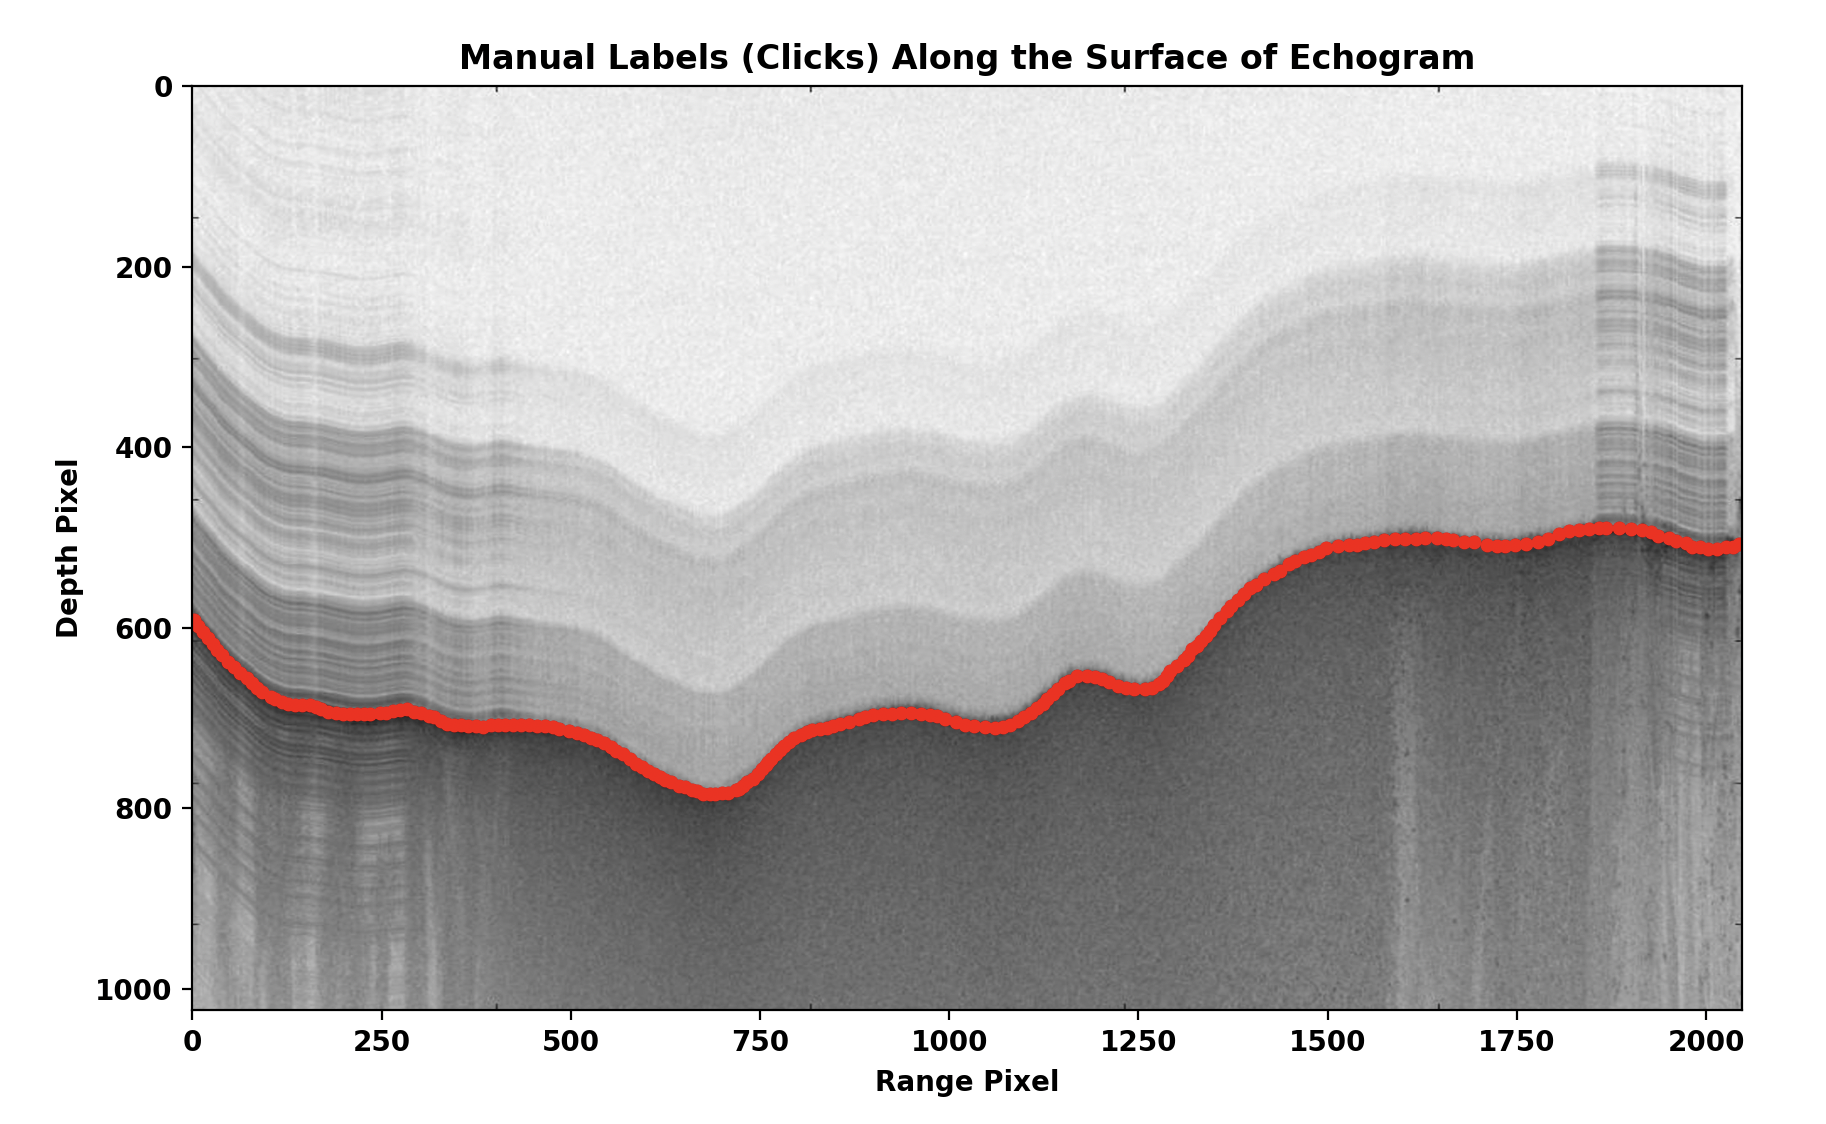
\includegraphics[width=0.9\textwidth]{figs/annotated_manual_label.png}
  \caption{Example of manual annotation via boundary clicks (no depth was labeled).}
  \label{fig:manual-label}
\end{figure}
The binary masked data (black color shows air and white color shows snow/ice) using two different labeling methods are shown in Figure~\ref{fig:labelling_data}. Notice that the manual label ignores minor noise whereas the weak label (script automated) shows minor variations (jitter) in air-snow boundary.\\\\
\textbf{Data Split:} The 30 processed echograms were split into three sets of 10:
\begin{itemize}[nosep]
  \item \textbf{\href{https://github.com/Mohammad-Neutrino/EECS836_Machine_Learning/tree/trunk/Project/data/labels_weak}{Weakly labeled set}}: used for initial model pretraining (\href{https://github.com/Mohammad-Neutrino/EECS836_Machine_Learning/blob/trunk/Project/src/generate_weak_labels.py}{generate\_weak\_labels.py})
  \item \textbf{\href{https://github.com/Mohammad-Neutrino/EECS836_Machine_Learning/tree/trunk/Project/data/labels_manual}{Manually labeled set}}: used for fine-tuning and internal validation \href{https://github.com/Mohammad-Neutrino/EECS836_Machine_Learning/blob/trunk/Project/src/manual_label_surface.py}{manual\_label\_surface.py}
  \item \textbf{Held-out set}: unseen during training, used for final evaluation
\end{itemize}
\begin{figure}[H]
  \centering
  
\includegraphics[width=0.45\textwidth]{figs/20220419_09_002_1echo.png}~~
  
\includegraphics[width=0.45\textwidth]{figs/20220427_01_006_1echo.png}
  \caption{Binary masking of echograms showing (Left)  Weak and (Right) Manual labels.}
  \label{fig:labelling_data}
\end{figure}

\section*{4. Method}
To perform surface segmentation on radar echograms, we adopt the U-Net architecture~\cite{1}, a popular convolutional neural network designed for semantic segmentation tasks. U-Net’s encoder–decoder structure makes it particularly well-suited for our application, where both local texture (e.g., surface edges) and global context (e.g., curvature across the frame) matter. The encoder progressively reduces the spatial resolution while learning increasingly abstract features, and the decoder upsamples these features back to the original resolution, allowing precise localization. Skip connections between corresponding encoder and decoder layers preserve fine-grained spatial information, which is crucial for maintaining boundary integrity in the output mask. As mentioned above, each input to the model is a preprocessed grayscale echogram image, and the output is a single-channel probability map of the same spatial dimensions. Each pixel in this map denotes the model's confidence that the corresponding input pixel belongs to the snow surface region.\\\\
\textbf{Loss Function:} We use a combination of Binary Cross Entropy (BCE) and Dice loss (DL) to guide training. BCE penalizes incorrect classifications at the pixel level, ensuring the model aligns tightly with surface boundaries. DL, on the other hand, measures the overlap between the predicted and true surface masks, helping improve performance in imbalanced regions where surface pixels are sparse relative to the background. The total loss is defined as:
\[
\mathcal{L} = 0.5 \cdot \text{BCE} + 0.5 \cdot \text{DL}
\]
This combined loss function proved effective in avoiding overfitting to smooth regions and reducing the ``hollow" effect observed in early-stage predictions, where the area under the surface boundary remained partially unfilled. Training was performed in two phases: an initial pretraining on weak labels to allow the model to learn general structural cues, followed by fine-tuning using a small set of manually labeled high-quality (and more reliable) annotations.\\\\
\textbf{Training Phases:}
\begin{itemize}[nosep]
  \item \textbf{Phase 1: Pretraining} on weak labels (5 epochs)
  \item \textbf{Phase 2: Fine-tuning} on manually labeled data (10 epochs)
\end{itemize}
\textbf{Execution:} The project is organized in a modular Python package on a GitHub repository (\texttt{\href{https://github.com/Mohammad-Neutrino/EECS836_Machine_Learning.git}{Mohammad-Neutrino/EECS836\_Machine\_Learning/Project/}}). Scripts can be executed directly from a terminal or in an IDLE. Throughout the report, the relevant scripts are mentioned in appropriate sections. In summary, the entire project requires executing the following scripts in this order:
\begin{itemize}[leftmargin=*]
  \item \texttt{preprocess.py}: crops and resizes echograms to \texttt{.npy} format
  \item \texttt{manual\_label\_surface.py}: interactive tool for manual boundary clicking
  \item \texttt{generate\_weak\_labels.py}: applies Sobel + Canny to generate weak labels
  \item \texttt{\href{https://github.com/Mohammad-Neutrino/EECS836_Machine_Learning/blob/trunk/Project/src/train.py}{train.py}}: performs pretraining and fine-tuning with live overlay generation
  \item \texttt{\href{https://github.com/Mohammad-Neutrino/EECS836_Machine_Learning/blob/trunk/Project/src/eval_metrics.py}{eval\_metrics.py}}: evaluates IoU/F1 on the manually labeled set
  \item \texttt{\href{https://github.com/Mohammad-Neutrino/EECS836_Machine_Learning/blob/trunk/Project/src/evaluate_heldout.py}{evaluate\_heldout.py}}: generates predictions on held-out echograms for generalization analysis
\end{itemize}

\section*{5. Experiments and Results}
All experiments were conducted on a remote cluster node, which was expected to provide GPU acceleration. However, due to environment configuration, the training defaulted to CPU usage. Despite this, the model was able to train efficiently: each epoch took approximately 2.5 minutes with a batch size of 2. Initially, we used only Binary Cross Entropy (BCE) loss, which encouraged precise pixel-level alignment with the weak labels. However, early results showed partially hollow patches in different regions, indicating that the model predicted sharp boundaries but failed to consistently fill the surface area beneath. To address this, we switched to a combined loss function consisting of BCE and DL. We used the Adam optimizer with a learning rate of $5 \times 10^{-4}$ across both training stages.\\\\
\textbf{Manual Set Evaluation:} 
To quantitatively assess performance, we evaluated the fine-tuned model on a set of 10 manually labeled echograms. Two standard segmentation metrics were used:
\begin{itemize}[noitemsep]
    \item \textbf{Intersection over Union (IoU):} Measures the overlap between predicted and true surface regions, defined as the ratio of their intersection to their union.
    \item \textbf{F1 Score:} The harmonic mean of precision and recall, which balances false positives and false negatives in the predicted mask.
\end{itemize}Both metrics were computed on binarized predictions and compared with the ground truth surface masks derived from manual clicks. Results are summarized in Table~\ref{tab:manual_eval} and visualized in Figure~\ref{fig:manual-barplot}. The model achieved consistently high IoU and F1 scores across the manual set, demonstrating that it effectively transferred knowledge learned from weak labels to precise boundary segmentation.


\begin{table}[H]
\centering
\caption{IoU and F1 Score on manually labeled echograms (\href{https://github.com/Mohammad-Neutrino/EECS836_Machine_Learning/tree/trunk/Project/data/labels_manual}{labels\_manual}). The model shows consistently high performance across all samples.}
\label{tab:manual_eval}
\vspace{0.5em}
\renewcommand{\arraystretch}{1.3} % Increase row spacing
\setlength{\tabcolsep}{12pt} % Increase column spacing
\begin{tabular}{|l|c|c|}
\hline
\textbf{Echogram} & \textbf{IoU} & \textbf{F1 Score} \\
\hline
20220427\_01\_006\_1echo & 0.889 & 0.941 \\
20220419\_04\_002\_1echo & 0.944 & 0.969 \\
20220419\_04\_007\_1echo & 0.984 & 0.992 \\
20220419\_04\_068\_1echo & 0.993 & 0.996 \\
20220419\_01\_008\_1echo & 0.996 & 0.998 \\
20220419\_04\_023\_1echo & 0.993 & 0.996 \\
20220419\_04\_070\_1echo & 0.992 & 0.996 \\
20220419\_04\_047\_1echo & 0.995 & 0.998 \\
20220419\_04\_037\_1echo & 0.995 & 0.997 \\
20220419\_01\_005\_1echo & 0.999 & 1.000 \\
\hline
\textbf{Mean} & \textbf{0.979} & \textbf{0.989} \\
\textbf{Standard Deviation} & \textbf{0.031} & \textbf{0.017} \\
\hline
\end{tabular}
\end{table}



\begin{figure}[H]
  \centering
  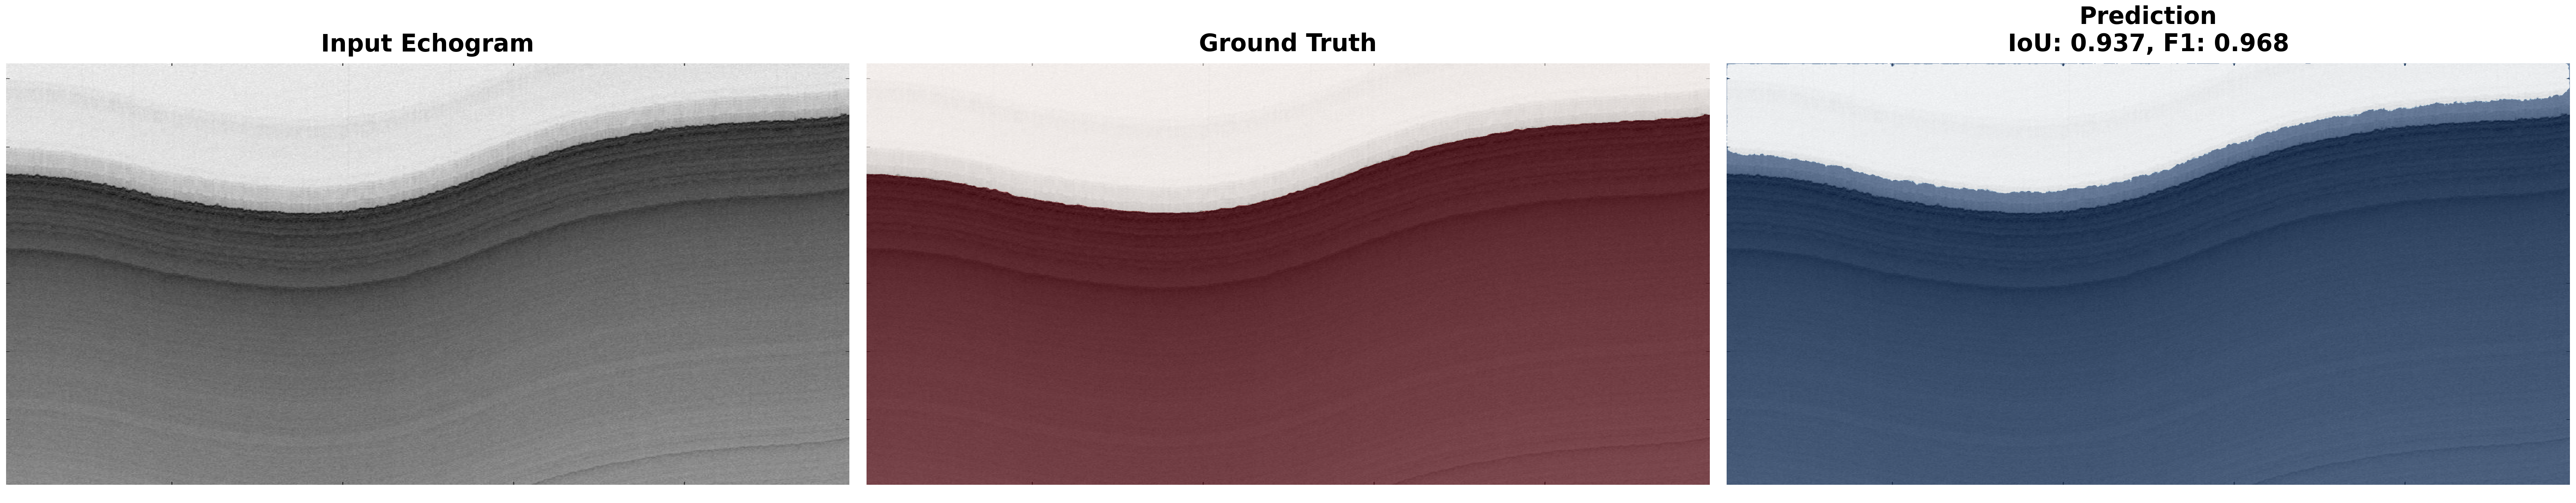
\includegraphics[width=0.95\textwidth]{figs/epoch1_sample0_1.png}
  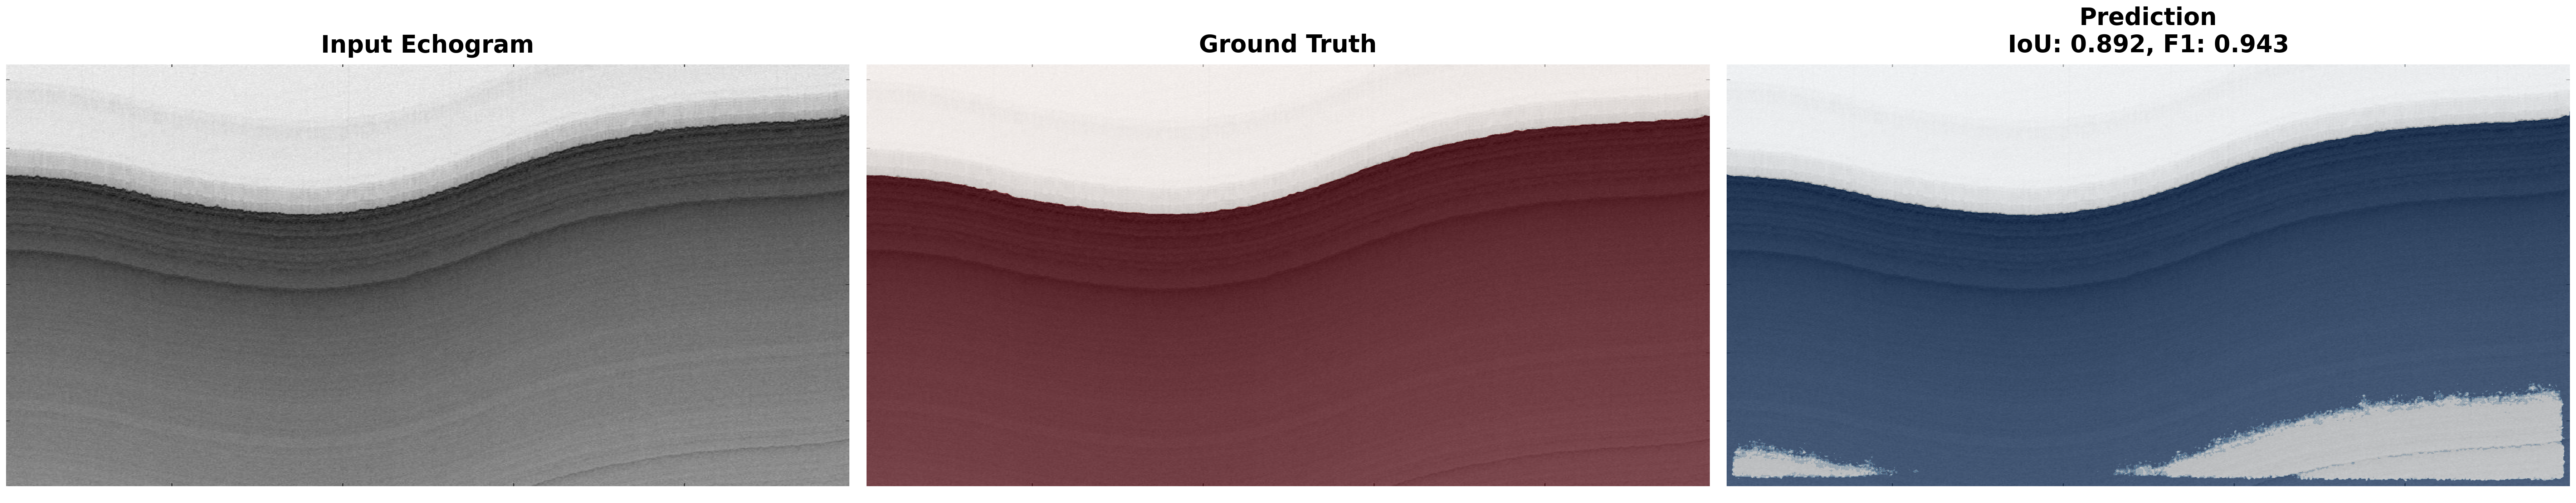
\includegraphics[width=0.95\textwidth]{figs/epoch6_sample2_1.png}
  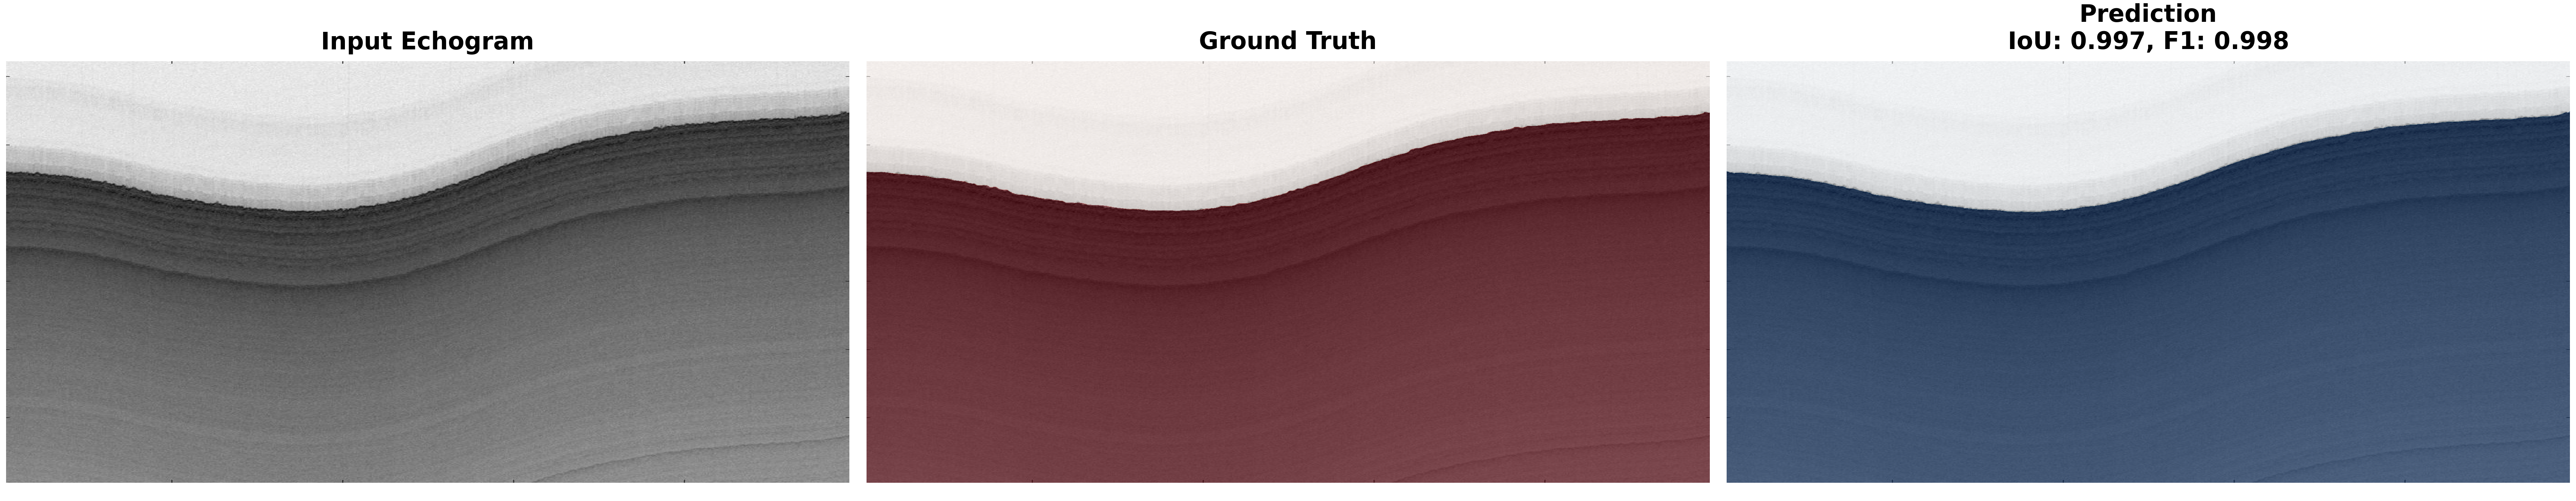
\includegraphics[width=0.95\textwidth]{figs/epoch10_sample0_1.png}
  \caption{Model predictions on the same echogram across different training epochs. Early predictions (Epoch 1) are complete and overfilled. Intermediate predictions (Epoch 6) shows ``hollow'' regions below the surface. Final epoch (Epoch 10) shows reasonably well recovery.}
  \label{fig:manual-hollow-evolution}
\end{figure}
To better understand how the model's predictions evolved during fine-tuning, we inspected prediction overlays on the same sample at multiple epochs. In the first epoch (Figure~\ref{fig:manual-hollow-evolution} {\bf top row}) following weak label pretraining, the model produced a rough but recognizable approximation of the air–snow boundary. The prediction covered more depth than necessary, resulting in a visibly thick segmented region. This was expected, as the weak labels encouraged general surface localization without precise depth control. By epoch 6 (Figure~\ref{fig:manual-hollow-evolution} {\bf middle row}), the model showed a curious artifact: although the air–snow boundary was clearly identified, a ``hollow" region appeared just beneath it. In this phase, the model seemed confident about the immediate boundary but uncertain about the filled-in snow region below, leading to inconsistent confidence across depth. This behavior did not persist and was not observed in most other samples or later epochs. By epoch 10 (Figure~\ref{fig:manual-hollow-evolution} {\bf bottom row}), the final prediction showed substantial improvement. The segmented surface region aligned closely with the ground truth, and the hollow pattern had disappeared. The predicted mask was both smooth and well-defined, indicating that the model successfully refined its understanding during fine-tuning. This transition across epochs demonstrates the effectiveness of combining weak label pretraining with a small set of manual annotations.

\begin{figure}[H]
  \centering
  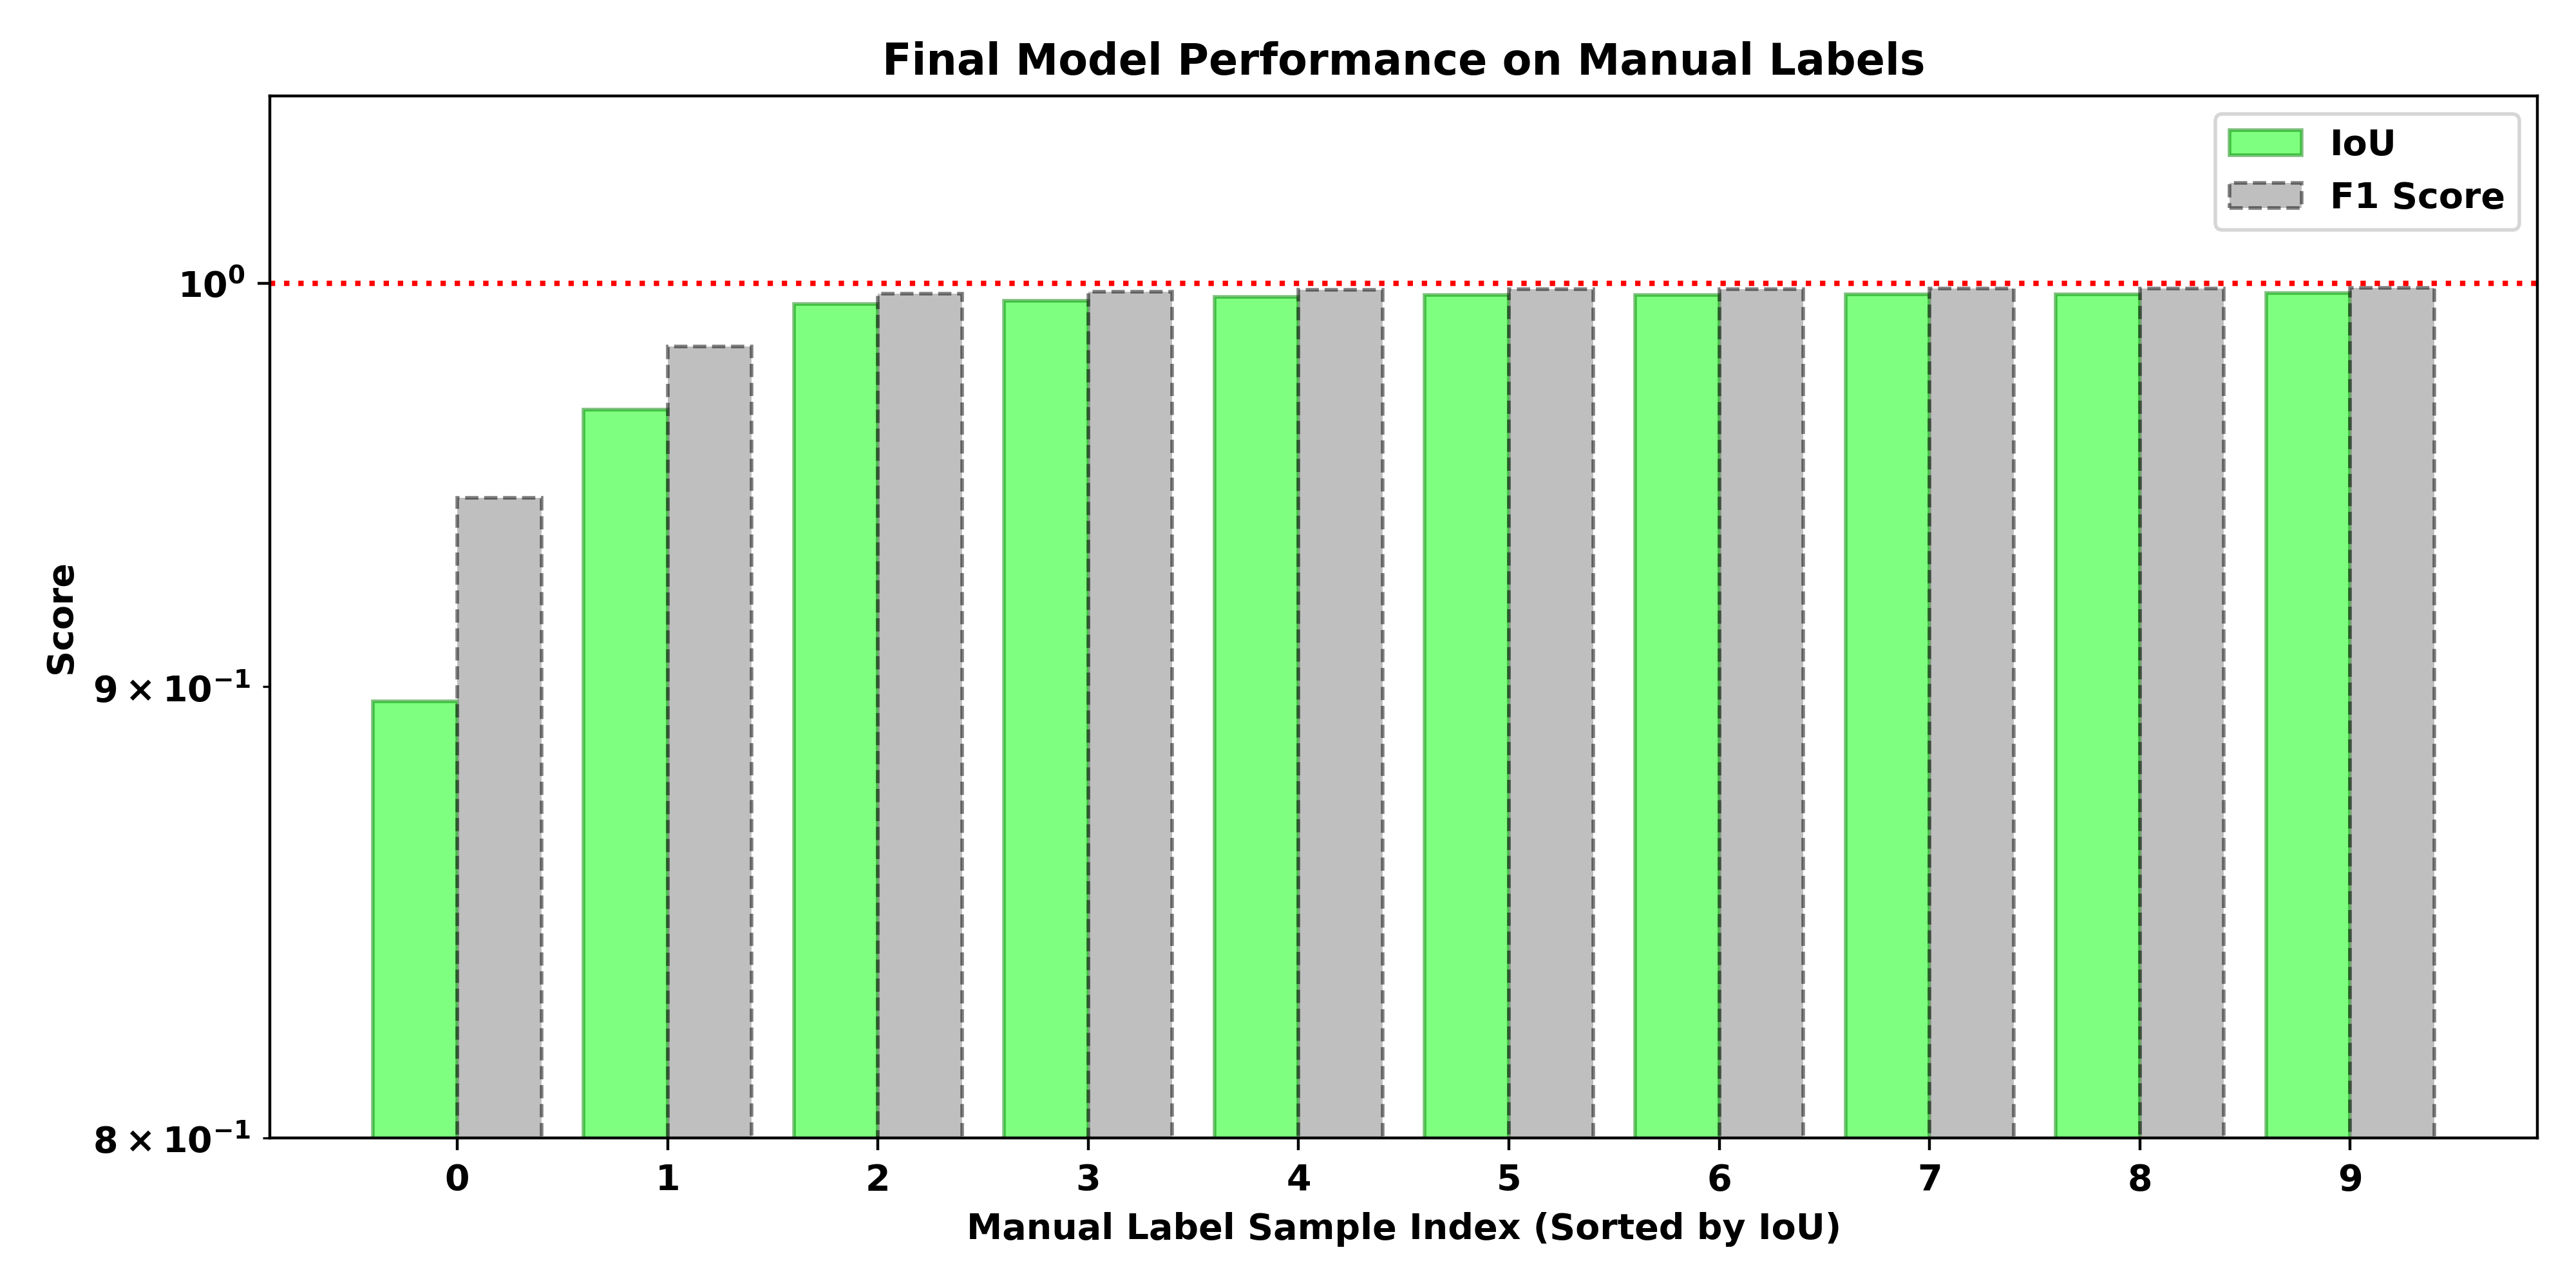
\includegraphics[width=0.85\textwidth]{figs/manual_set_performance.png}
  \caption{Sorted IoU and F1 scores on manually labeled set (log scale).}
  \label{fig:manual-barplot}
\end{figure}
\begin{figure}[H]
  \centering
  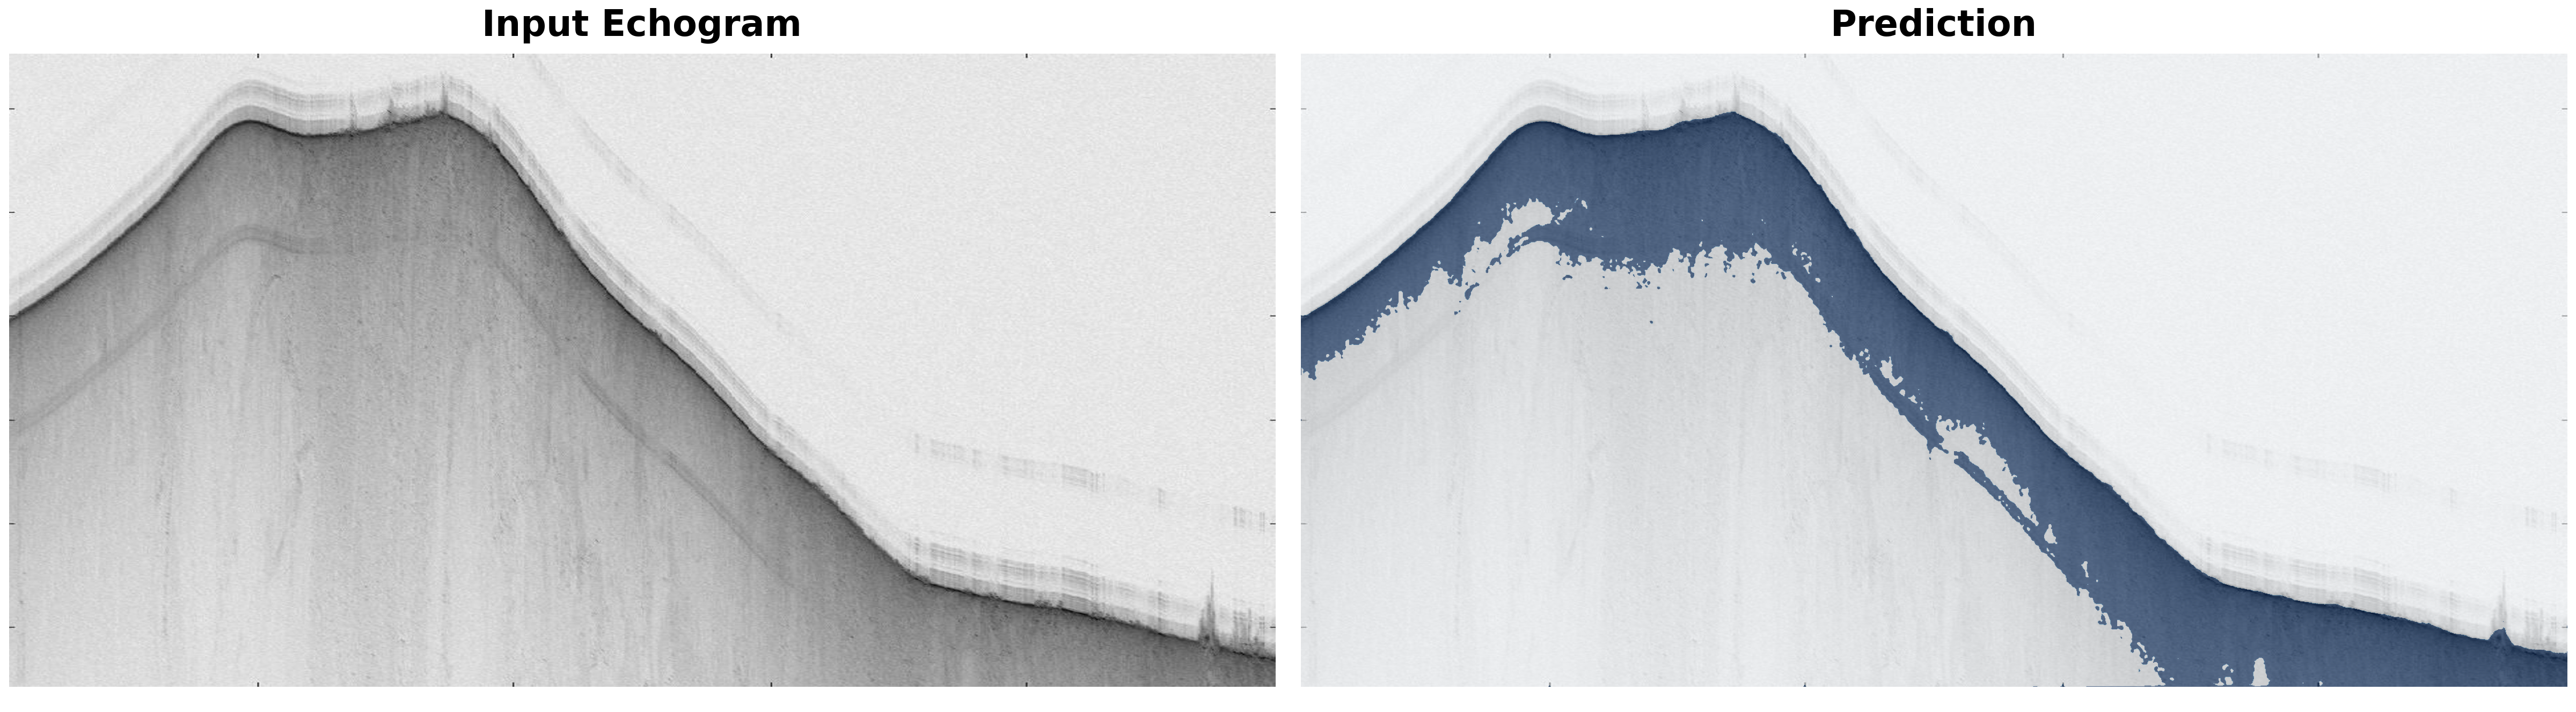
\includegraphics[width=0.95\textwidth]{figs/20220427_01_004_1echo.png}
  \caption{Prediction on a held-out echogram with noisy and non-uniform layering.}
  \label{fig:heldout-robust}
\end{figure}
\textbf{Held-Out Evaluation:}
Figure~\ref{fig:heldout-robust} presents a held-out example that highlights the model’s robustness in noisy or less structured echograms. Despite the absence of clean, layered stratigraphy typically observed in easier examples, the model correctly identifies the approximate location of the snow-air boundary. The prediction displays slight over-segmentation and spatial jitter, particularly in the central region, but still tracks the general curvature of the surface well. This example underscores the benefit of pretraining with weak labels, which appears to have helped the model generalize to surface textures that differ significantly from the manually labeled fine-tuning set.

\section*{6. Conclusion and Future Prospects}
This project developed an efficient pipeline to segment air–snow interfaces in radar echograms using minimal supervision. By combining weak label pretraining with manual fine-tuning, we achieved strong performance with minimal annotation effort. The model learned to generalize across held-out samples, though occasional over-segmentation or ``hollow" predictions were observed.\\\\
Moving forward, the methodology can be extended in several ways. The original CReSIS data includes \texttt{.mat} files containing raw radar return amplitudes, GPS coordinates, elevation models, and frame metadata. Leveraging this richer information would allow not only better echogram rendering but also geospatial surface mapping, time-series tracking of snow accumulation, and potentially even 3D surface reconstruction when used in conjunction with position data. On the image side, several enhancements are possible. Applying temporal context (e.g., using neighboring echograms in sequence) could stabilize noisy predictions, while incorporating post-processing (like morphological filters) could clean up false positives. Using active learning, the model could identify uncertain regions to prioritize for manual labeling, further reducing annotation load.\\\\
Most importantly, once trained, the model can be deployed to segment air–snow boundaries across vast radar datasets collected in Greenland, Antarctica, and other regions without the need for location-specific retraining. This opens the door to scaling up snow layer analysis across campaigns and years, supporting long-term climate monitoring and accumulation modeling at polar scales.


\bibliographystyle{unsrt}
\begin{thebibliography}{1}
\bibitem{1}{Ronneberger, O., Fischer, P., \& Brox, T. (2015). U-Net: Convolutional networks for biomedical image segmentation, MICCAI 2015, \href{https://arxiv.org/abs/1505.04597}{https://arxiv.org/abs/1505.04597}.}
\bibitem{2}{Crandall, K. C., et al. (2016). Layer identification and tracking in radar echograms using probabilistic graphical models, \textit{IEEE Transactions on Geoscience and Remote Sensing}.}
\bibitem{3}{Zhang, H., et al. (2021). Weakly supervised semantic segmentation with segment-based consistency loss. \textit{CVPR 2021}.}
\bibitem{4}{MacGregor, J. A., et al. (2015). Radiostratigraphy and age structure of the Greenland Ice Sheet. \textit{Journal of Geophysical Research: Earth Surface}.}
\bibitem{5}{CReSIS: Center for Remote Sensing of Ice Sheets, \href{https://data.cresis.ku.edu/data/snow/}{CReSIS Snow Radar Dataset}.}
\end{thebibliography}
\end{document}

